\documentclass{article}

\usepackage{ctex}
\usepackage[left=1.25in,right=1.25in,top=1in,bottom=1in]{geometry}
\usepackage{amsmath}
\usepackage{amssymb}
\usepackage{graphicx}
\usepackage{float}
\usepackage{subfigure}
\usepackage{listings}
\usepackage{xcolor}
\lstset{language=Python}   
\lstset{breaklines}              
\lstset{extendedchars=false}
\lstset{ 
	backgroundcolor=\color{white},   % 选择代码背景,必须加上\ usepackage {color}或\ usepackage {xcolor}.
	basicstyle=\footnotesize,        % 设置代码字号.
	breakatwhitespace=false,         % 设置是否当且仅当在空白处自动中断.
	breaklines=true,                 % 设置自动断行.
	captionpos=b,                    % 设置标题位置.
	commentstyle=\color{mygreen},    % 设置注释格式
	deletekeywords={...},            % 是否删除给定语言的关键词.
	escapeinside={\%*}{*)},          % 是否在代码中添加LaTex.
	extendedchars=true,              % 是否允许使用非ASCII字符; 仅适用于8位编码,不适用于UTF-8. 
	frame=single,	                   % 给代码区添加边框.
	keepspaces=true,                 % 保留空格(useful for keeping indentation of code (possibly needs columns=flexible).
	keywordstyle=\color{blue},       % 关键字显示风格.
	language=Octave,                 % 使用的语言.
	morekeywords={*,...},            % 是否需要添加其他的关键词.
	numbers=left,                    % 给代码添加行号,可取值none, left, right.
	numbersep=5pt,                   % 设置行号与代码之间的间隔
	numberstyle=\tiny\color{mygray}, % 行号的字号和颜色
	rulecolor=\color{black},         % 边框颜色,如果没有设置,框架颜色可以在非黑色文本中的换行符上更改(例如 text (e.g. comments (green here)))
	showspaces=false,                % 显示每个地方添加特定下划线的空格; 覆盖了'showtringspaces'
	showstringspaces=false,          % 仅在字符串中允许空格
	showtabs=false,                  % show tabs within strings adding particular underscores
	stepnumber=2,                    % the step between two line-numbers. If it's 1, each line will be numbered
	stringstyle=\color{mymauve},     % string literal style
	tabsize=2,	                   % 将默认tab设置为2个空格
	title=\lstname                   % show the filename of files included with \lstinputlisting; also try caption instead of title
}

\usepackage[framed,numbered,autolinebreaks,useliterate]{mcode}

\author{张泽宇}
\date{2022年6月5日}
\title{第十二至第十五周工作总结}

\begin{document}
	\maketitle
	
	{\centering \rule[15pt]{15cm}{0.1em}}
	
	{
		\noindent
		\large
		\textbf{过去四周的主要进行的工作包括有:
			\begin{itemize}
				\item 针对仿真模型,增加了故障发生时间和故障过渡电阻两个变量,模拟更多种情况。
				\item 针对仿真数据,选取故障发生时两个周期波形以及故障前后各半周波形作为网络输入,将灰度图大小调整到16$\times$16像素。
				\item 针对神经网络模型,在之前基础上调整了一些参数,简化了网络构造。
			\end{itemize}
	}}
	
	以下为详细叙述
	
	{\centering \rule[-10pt]{15cm}{0.1em}}
	
	\newpage

	
	\section{仿真模型修改}
	
	仿真模型改动如下:
	
	\subsection{故障发生时间设为变量}
	
	用 FaultTime 表示故障发生时间,利用Multiple Run模块控制其从0.05s开始,以0.02步长变化至0.15s;同时,调节模型的采样时间为0.5ms,即采样频率为2000Hz。
	
	\subsection{故障电阻阻值设为变量}
	
	用 TransitionR 表示故障电阻的阻值,利用Multiple Run模块控制其值依次选取750$\Omega$、1000$\Omega$和1250$\Omega$。
	
	需要注意的是,这里无论是FaultTime的取值还是TransitionR的取值,都可以再做更多细分,从而获得更多的实验数据。但是为简便起见,这里只得出72组原始数据,在通过后期数据增强,拓展数据集。
	
	\begin{figure}[h]
		\centering
		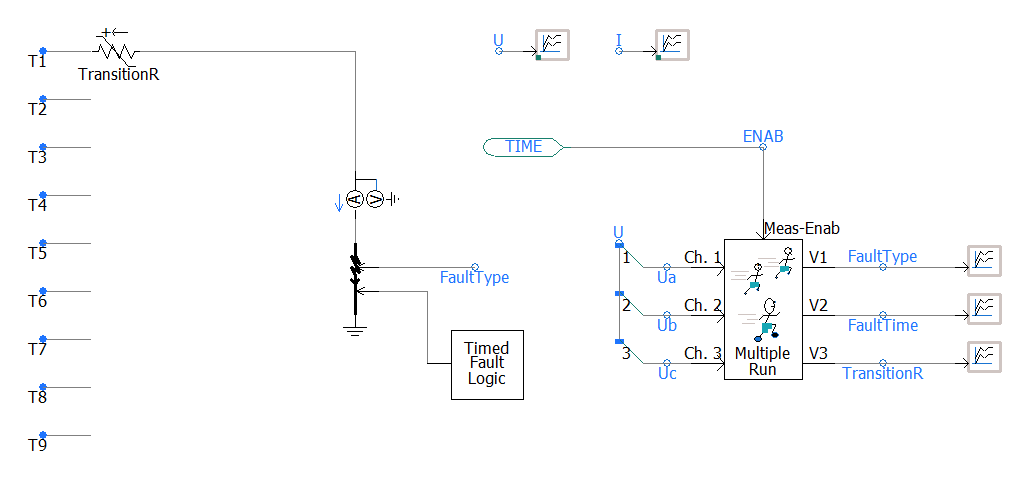
\includegraphics[width=14cm]{figure/1.png}
		\caption{修改后的仿真控制部分}
	\end{figure}
	
	\section{仿真数据处理}
	
	听取李教授的建议,将输入模型的数据减少。选取故障时两个完整波以及故障前后各半波数据作为输入,生成16$\times$16的灰度图。由于采样频率是2000Hz,在一个完整波上有40个数据点,因此一共有120个数据点,考虑到三相输入,共有360个数据点。而16$\times$16像素灰度图需要256个数据点,因此无论怎样截取数据,都可以使生成的灰度图中包含正常数据与故障数据,且故障数据一定占据大多数。从而各个故障种类灰度图之间存在一定的差距。而且从最后的结果来看,这样处理达到了和之前128$\times$128像素灰度图一样的识别结果。
	
	同时,还对原来读取PSCAD数据,生成灰度图的程序进行了优化和完善,体现在用os库的一些函数修改原先的路径设计、减少了for循环的个数,提高程序效率、合并了一些函数。
	
	修改后的代码上传在了Github上,可进行下载修改。
	
	最终得到的灰度图像如下图所示:
	
	\begin{figure}[ht]
	\centering
	\subfigure{
		\begin{minipage}[t]{0.4\linewidth}
			\centering
			
\includegraphics[width=2in]{figure/2.jpg}
			\caption{A相短路接地}
		\end{minipage}
	}
	\subfigure{
		\begin{minipage}[t]{0.4\linewidth}
			\centering
			
\includegraphics[width=2in]{figure/3.jpg}
			\caption{AB相短路接地}
		\end{minipage}
	}
	
	\subfigure{
		\begin{minipage}[t]{0.4\linewidth}
			\centering
			
\includegraphics[width=2in]{figure/4.jpg}
			\caption{ABC三相短路接地}
		\end{minipage}
	}
	\subfigure{
		\begin{minipage}[t]{0.4\linewidth}
			\centering
			
\includegraphics[width=2in]{figure/5.jpg}
			\caption{AB相短路}
		\end{minipage}
	}
	
	\end{figure}
	
	\section{神经网络模型的修改}
	
	传统的的LeNet-5网络中,由于输入的图像为32像素;之前的神经网络输入为128像素,因此不需要过多考虑卷积和池化对图像大小的影响。但是对于16像素的输入,如果延续之前的结构,在第二次卷积后就变为5像素的特征图,再进行池化,担心特征图太小,导致特征丢失。所以,将第二层池化去掉,卷积之后直接连接全连接层。
	
	网络模型及参数如下图:
	
	\begin{figure}
		\centering
		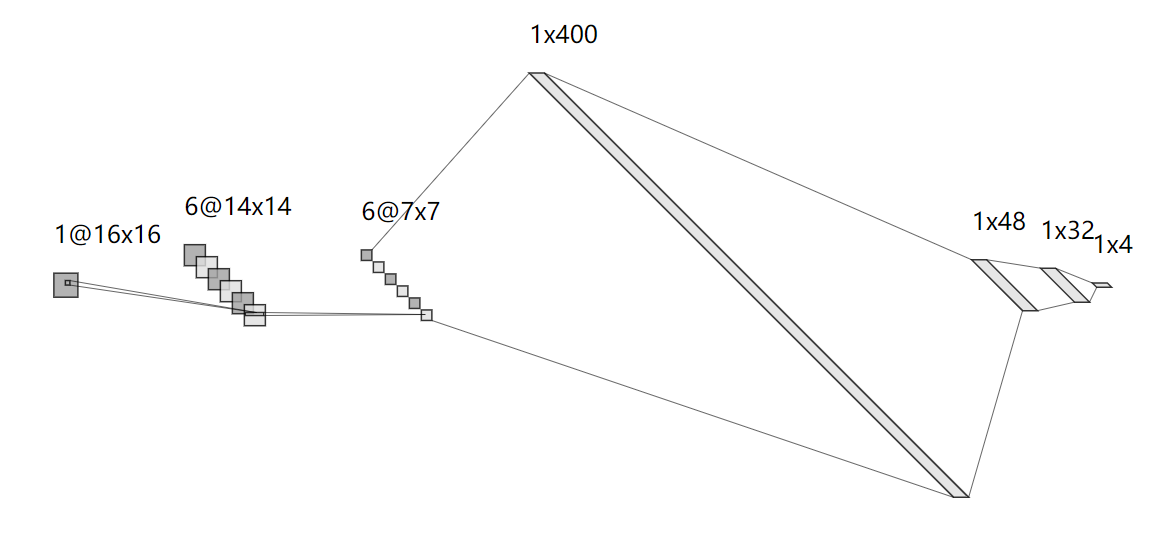
\includegraphics[width=10cm]{figure/9.png}
		\caption{网络模型}
	\end{figure}
	
	基于修改后的神经网络模型,进行训练。训练集:验证集为5:1,即6000张训练集,1200张验证集;学习率为0.01,训练10轮,采用随机梯度下降法进行优化,采用交叉熵计算训练损失,训练过程中的训练损失函数、验证损失函数、正确率测试变化如图7至图9所示:
	
	\begin{figure}[h]
		\centering
		\subfigure{
			\begin{minipage}[t]{1\linewidth}
				\centering
				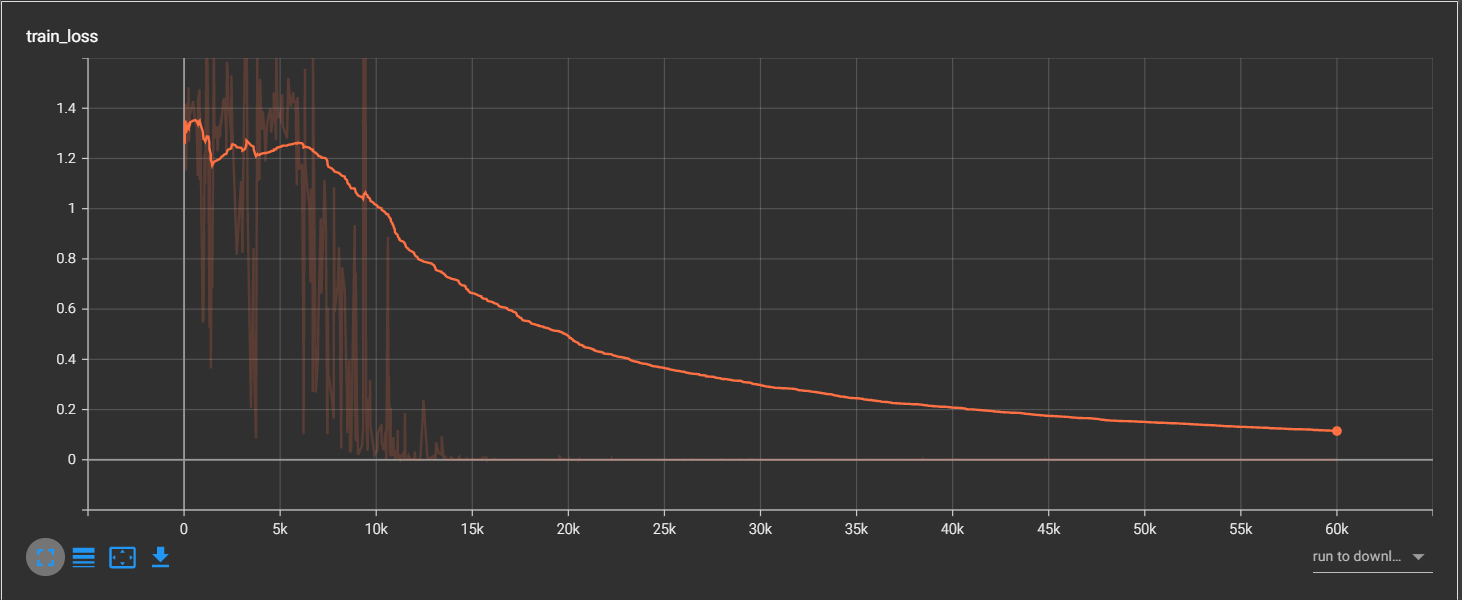
\includegraphics[width=13cm]{figure/6.png}
				\caption{训练损失函数}
			\end{minipage}
		}
	
		\subfigure{
			\begin{minipage}[t]{1\linewidth}
				\centering
				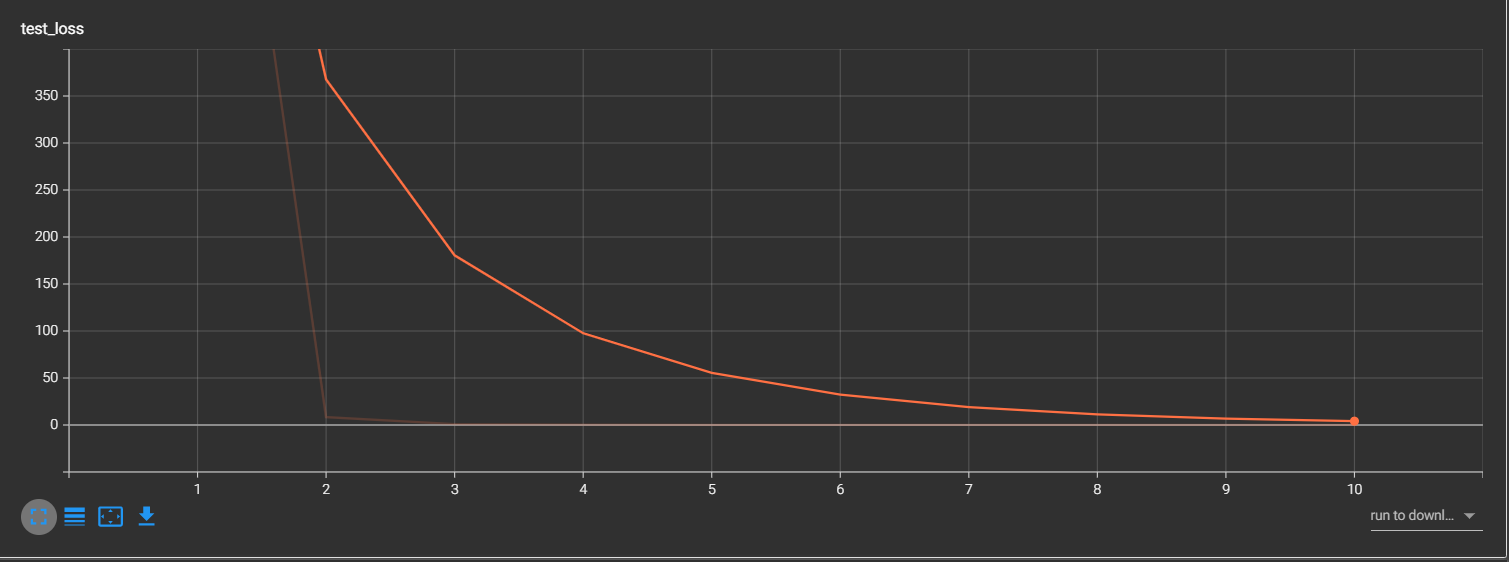
\includegraphics[width=13cm]{figure/8.png}
				\caption{验证损失函数}
			\end{minipage}
		}
		
		\subfigure{
			\begin{minipage}[t]{1\linewidth}
				\centering
				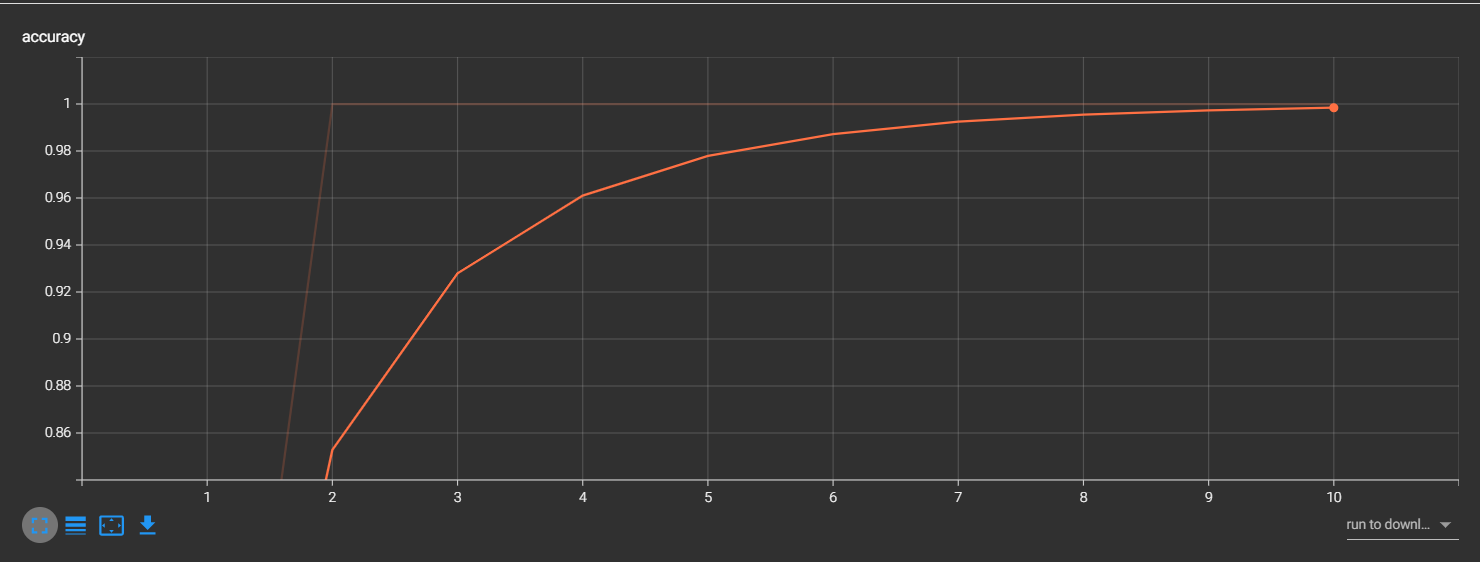
\includegraphics[width=13cm]{figure/7.png}
				\caption{正确率测试}
			\end{minipage}
		}
		
	\end{figure}
	
	根据未拟合的图像(即浅黄色图像),可以看出10论训练之后损失函数已经接近于0,而正确率达到100\%,由输出的数据显示,最后一轮训练的损失值为8.344646857949556e-07。
	
	经过测试程序的验证,发现模型达到了故障类别识别的效果。
	
	综上所述,模型实际上达到的效果与之前模型一样,但是明显的是这个模型无论是在数据大小还是训练速度上都更优,说明选择合适的数据输入大小对于模型来说是十分重要的,在保证不失真和不遗漏特征的前提下,尽可能的减少模型输入数据,从而节省算力。
	
	以上模型代码可在Github主页上找到,这里就不占较多篇幅展示。
	
	
	在过去的一个月中,由于一些课程的课程论文以及学院活动的影响,所以取得的进展不是很多。大多是一些总结和对之前细节的修修补补,接下来的一个月因为期末考试的缘故,能够分配的时间也不是太多。所以大刀阔斧的修改和完善只能等到期末结束之后再进行。
	
\end{document}